% $Id$
\documentclass[twocolumn,prd,nofootinbib]{revtex4}


\newcommand\ForInternalReference[1]{}
\newcommand\SkipForEarlyCirculation[1]{}
\newcommand\AddedResponse[1]{{\color{blue} {#1}}}
%\newcommand\SkipForEarlyCirculation[1]{#1}
\newcommand\SkipPP[1]{}
\usepackage{verbatim}
\usepackage{graphicx}
\usepackage{dcolumn}
\usepackage{bm}
\usepackage{color}
\usepackage{xspace}
\usepackage{url}
\usepackage{amsmath}
%\usepackage{adjustbox}
\usepackage{float}
\usepackage{multirow}
\usepackage{amssymb}
%
%
\usepackage{times}
%
%
%
\newcommand\optional[1]{}

%
\newcommand\E[1]{\left\langle #1\right\rangle}
\newcommand\qmstate[1]{\left|#1\right \rangle}
\newcommand\qmstateKet[1]{\left\langle#1\right|}
\newcommand\qmstateproduct[2]{\left\langle#1|#2\right\rangle}
\newcommand\qmoperatorelement[3]{\left\langle#1\left|#2\right|#3\right\rangle}
\newcommand\qmoperator[1]{{\bf #1}}
%
\newcommand\Y[1]{{{}_{#1}Y}}

\newcommand\lnL{ \ln {\cal L}}
\newcommand\lnLmarg{ \ln{\cal L}_{\rm marg}{}}
\newcommand\unit[1]{{\rm #1}}

\newcommand\rapidPEOrig{rapid\_pe1}
\newcommand\ILE{ILE}
\newcommand\editremark[1]{{\color{red} #1}}
%
%
%
\usepackage{color}
\definecolor{amber}{rgb}{1.0, 0.75, 0.0}
\definecolor{orange}{rgb}{1.0, 0.5, 0.0}
\definecolor{amaranth}{rgb}{0.9, 0.17, 0.31}
\def\fixme#1{\textcolor{red}{#1}}
\newcommand{\Richard}[1]{ {\color{blue}{#1}}}
\newcommand{\ros}[1]{ {\color{blue}{#1}}}
%

%

%
%
%
%
\graphicspath{{./figures/}}
\newcommand{\mc}{{\cal M}}
\newcommand{\Ms}{M_{\odot}}
\newcommand\LambdaTilde{\widetilde{\Lambda}}
\newcommand\DeltaLambdaTilde{\delta \widetilde{\Lambda}}
%
\def\ltsima{$\; \buildrel < \over \sim \;$}
\def\simlt{\lower.5ex\hbox{\ltsima}}
\def\gtsima{$\; \buildrel > \over \sim \;$}
\def\simgt{\lower.5ex\hbox{\gtsima}}

\newcommand\prx{Phys.~Rev.~X}
\def\aj{Astronomical Journal}                 %
\def\apj{Astrophysical Journal}                %
\def\apjl{Astrophysical Journal}             %
\def\pasj{PASJ}
\def\apjs{ApJS}              %
\def\mnras{MNRAS}            %
\def\prd{Phys.~Rev.~D}       %
\def\prl{Phys.~Rev.~Lett}    %
\def\cqg{Class.~Quant.~Grav.~}%
\def\araa{ARA\&A}             %
\def\nat{Nature}              %
\def\aap{A\&A}                %
\def\aapr{A\&A~Rev.~}    %
\def\pasp{PASP}    %
\def\sovast{Soviet Ast.}
%
%

\newcommand{\IMRPD}{\textsc{IMRPhenomD}\xspace}
\newcommand{\IMRPDT}{\textsc{IMRPhenomD\_NRTidal}\xspace}
\newcommand{\IMRP}{\textsc{IMRPhenomPv2}\xspace}
\newcommand{\SEOBP}{\textsc{SEOBNRv3}\xspace}
\newcommand{\SEOBA}{\textsc{SEOBNRv4}\xspace}
\newcommand{\SEOBAROM}{\textsc{SEOBNRv4\_ROM}\xspace}
\newcommand{\NRSur}{NRSur7dq2\xspace}
\newcommand{\TEOB}{SEOBNRv4T\xspace}
\newcommand{\Resum}{TEOBResumS\xspace}
\newcommand\RIFT{RIFT}
\newcommand{\Taylor}{TaylorF2\xspace}
\newcommand\PaperDetection{\underline{LVC-detect}\cite{DiscoveryPaper}}
\newcommand\PaperPE{\underline{LVC-PE}\cite{PEPaper}}
\newcommand\PaperTestGR{\underline{LVC-TestGR}\cite{TestingGRPaper}}
\newcommand\PaperPENRMethods{\underline{PE+NR-Methods}\cite{gwastro-PENR-Methods-Lange}}
\newcommand\PaperAstro{\underline{LVC-Astro}\cite{AstroPaper}}
\newcommand\PaperBurst{\underline{LVC-Burst}\cite{BurstPaper}}
\newcommand\PaperRates{\underline{LVC-Rates}\cite{RatesPaper}}
\newcommand\PaperStochastic{\underline{LVC-Stochastic}}
\newcommand\PaperSEOBNRvthree{\underline{LVC-SEOBNRv3}\cite{SEOBv3Paper}}

\def\RIT{Center for Computational Relativity and Gravitation, Rochester Institute of Technology, Rochester, New York 14623, USA}

\begin{document}

\title{Population Inference of Non-Spinning Eccentric Binary Black Holes}
\author{M. Zeeshan}
\affiliation{\RIT}
\author{R. O'Shaughnessy}
\affiliation{\RIT}
\begin{abstract}
Yet to work. 
\end{abstract}
\maketitle

\section{Introduction}
Big Picture
\begin{itemize}
    \item GWs are important
    \item ecccentricity is a signature that can be measued with GWs
    \item it is a unique signature of strong events
\end{itemize}
Why Population, smaller picture
\begin{itemize}
    \item population inference of eccentricity is important.
    \item some events may have unabmoguis eccentricty (refs to PE, richard will send them), but many will have only faint signatures or none at all.
    \item critical for astrophysoics to acces distribution of eccentricites and any subpopulation
\end{itemize}
Previous work
\begin{itemize}
    \item What other people have done with eccentricty, 
    \item cite any preious work realted to eccentricty with population.
    \item mostly it's real events or high mass evenets
    \item what sort of eccentricy we expect to appear
\end{itemize}
\begin{itemize}
    \item Explain,what and how you are doing here.
    \item assess how well eccentricity of population  can be inferreed using low mass BHS where eccentricity measurement should be much more precise.
    \item for simplicity using a proof of concept population model to emphasize eccentric inference
\end{itemize}

We discussed the various formation scenario of EBBHs in the previous section; each one has a distinct signature in the GW signals. Hence, it's trivial to observe the effect of each scenario or the mixed effect on the merging population. It leads us to make the population model, which considers each scenario and allows distinct merger rates for them.

Most of the eccentric binary black hole (EBBHs) are driven by low masses $(10M_\odot-30M_\odot)$ and if any component of the binary have mass less than $30 M_\odot$ then only $10\%$ of them are able to maintain eccentricity near the last stable orbit.  \cite{mass_ecc_limit_2018}. Therefore,  in this study, we  will consider binaries with non-spinning $(\chi_i = 0)$, eccentric $(0-0.5)$ and moderate mass range $(10M_\odot-50M_\odot)$. In addition, we will use mass ratio $q=m_1/m_2$ with condition $m_1>m_2$ and total mass $M=m_1+m_2=100M_\odot$.



\section{Methods}
\label{sec:methods}

The coalescing BBH can be completely described by three intrinsic and seven extrinsic parameters. The intrinsic parameters mass of binary component ($m_i$), spin $( \chi_i)$, and eccentricity $\epsilon$  are subject to the orbital evolution of the binary. The extrinsic parameters are orientation (orbital phase, polarization, and inclination), sky location (right ascension and declination), luminosity distance, and coalescence time depend on the observer.



\subsection{Hierarchical Bayesian Modeling (HBM)}



Once we have the population models, our next obstacle is constraining them with observational data. While constraining the model, we must consider the sensitivity of LIGO-VIRGO-KAGRA (LVK) and uncertainty in each detection. Therefore, the HBM is a good choice to constrain the population model.

In the HBM, we have the N number of discrete detection, in our case, from LVK. Those detections provide merger data denoted as $d_1,d_2,d_3,...,d_N$ where each $d_i$ shows the BBH. Each $d_i$ or merger has mass, spin, and eccentricity properties. These properties, often called parameters, are denoted by $\lambda_1,\lambda_2,\lambda_3,...,\lambda_i$. Each parameter has its uncertainty, and we express it by the probability of the data given the parameter value. We also refer to it as the likelihood function $\mathcal{L}(\lambda)=p(d|\lambda)$ of one event/detection. The given value of $\lambda$ to calculate the likelihood is obtained from the mathematical model of the waveform. Once you have a likelihood function, you can use a prior (usually, a uniform) to find the posterior probability using the Bayes theorem.

\begin{equation}
\label{eq:Bayes_ind}    
p(\lambda|d) \propto p(d|\lambda) p(\lambda)
\end{equation}

This posterior probability will constrain the properties of each binary, such as mass, spin, and eccentricity. We may get the inference of those parameters using Rapid parameter Inference on gravitational wave sources via Iterative Fitting (RIFT): an open source code for parameter estimation of the binary sources \cite{rift_2018}.



%\begin{itemize}
%    \item We have N discrete detection.
%    \item each detection has data $d_1,d_2,d_3,...,d_N$
%    \item each data point $d_N$ has properties denoted by $\lambda_1,\lambda_2,...,\lambda_i$
%    \item  $ \lambda_i$ are parameters such as mass, spin, eccentricity, and location.
%    \item Each parameter has its uncertainty.
%    \item This uncertainty is described by the probability of the data given the parameter value. We call it the likelihood function of one single event. $\mathcal{L}(\lambda) = p(d|\lambda)$
%    \item the waveform gives the parameter value.
%    \item waveform is a mathematical function.
%    \item Once you have a likelihood function, you can use prior( usually it's uniform: which gives equal probability to each event) to find the posterior. $p(\lambda|d) \propto p(d|\lambda) p(\lambda)$  
    
%\end{itemize}


\subsection{Population Inference}

Now having the parameters of individual sources, we are ready to make a population inference. Following the Bayesian framework for inference, our first task is to find the likelihood of the population parameter $\Lambda$, also considered as uncertainty in $\Lambda$ equivalent to the probability of the individual sources given the population parameter $\Lambda$ written as follows. 

\begin{equation}
\label{eq:likelihood_pop}    
\mathcal{L}(\Lambda)\equiv p(d_1,d_2,d_3,...,d_N|\Lambda)
\end{equation}

 

The second step is to find the posterior probability, and we can do this by using the above likelihood in the Bayes theorem as given below.

\begin{equation}
\label{eq:Bayes}    
p(\Lambda|d_1,d_2,...,d_N)= \frac{p(\Lambda)p(d_1,d_2,...,d_N|\Lambda)}{p(d_1,d_2,...,d_N)}
\end{equation}

where $p(\Lambda|d_1,d_2,d_3,...,d_N)$ is posterior, $p(\Lambda)$ is prior, $p(d_1,d_2,d_3,...,d_N)$ is normalization constant or sometime known as evidence.

To conduct our specific analysis for mass and eccentricity distribution, we will use the inhomogeneous Poisson Process scaled by rate $\mathcal{R} = \frac{dN}{dtdV_c}$ and parameterize by $\Lambda$ to find the likelihood  $\mathcal{L}(\mathcal{R},\Lambda)\equiv p(D|\mathcal{R},\Lambda)$ of an astrophysical population given the merger rate and parameter $\Lambda$. 

\begin{equation}
\label{eq: likelihood}
\mathcal{L}(\mathcal{R},\Lambda) \propto e^{-\mu(\mathcal{R},\Lambda)}\prod_{n=1}^N\int d\lambda \ell_n(\lambda) \mathcal{R} p(\lambda|\Lambda),
\end{equation}

Where $\mu(\mathcal{R},\Lambda)$ is the expected number of detection under the given population parametrization $\Lambda$ with the overall rate $\mathcal{R}$. $\ell_n(\lambda)=p(d_n|\lambda)$ is the likelihood of the data $d_n$ given binary parameter.
Finally, we will get our posterior as $p(\mathcal{R},\Lambda)\propto p(\mathcal{R},\Lambda)  \mathcal{L}(\mathcal{R},\Lambda)$.

These calculations are analytically intractable and must be performed numerically. Specifically, we will use Goodman and Weare's affine invariant Markov chain Monte Carlo (MCMC) \cite{mcmc_paper} method to find the posterior distribution of population parameters. This method draws samples from the targeted distribution for $\Lambda$; in our case, it's the power law model given in Eq. \ref{eq:plawg}, then compares it with the given data (collection of individual events) and store the best-fit sample. We may iterate this as we need and store multiple sample values untill they converge. 
This method is in a Python package called EMCEE \cite{emcee_paper}.





%\begin{itemize}
%    \item We have the parameter estimation from RIFT or any other method. It will give us a distribution for each parameter, and we may take the mean value of it.
 %   \item Our first task is to find the likelihood function for the population parameters: such as mass and eccentricity.
%    \item We denote population parameters with \\ $\Lambda \equiv  (\alpha, \mathcal{R}, m_{min}, m_{max}, e)$.
%    \item uncertainty in $\Lambda$ is a likelihood which can be written as $\mathcal{L}(\Lambda)\equiv p(d_1,d_2,d_3,...,d_N|\Lambda)$
%    \item By applying the Bayes theorem, we can turn above likelihood into posterior probability of a parameter.
%\begin{equation}
%\label{eq:Bayes}    
%p(\Lambda|d_1,d_2,...,d_N)= \frac{p(\Lambda)p(d_1,d_2,...,d_N|\Lambda)}{p(d_1,d_2,...,d_N)}
%\end{equation}

%    \item where $p(\Lambda|d_1,d_2,d_3,...,d_N)$ is posterior, $p(\Lambda)$ is prior, $p(d_1,d_2,d_3,...,d_N)$ is normalization/evidence, and $p(d_1,d_2,d_3,...,d_N|\Lambda)$ is likelihood.
 
%   \item We will use inhomogeneous Poisson Process scaled by rate $\mathcal{R} = \frac{dN}{dtdV_c}$ and parameterize by $\Lambda$ to find the likelihood  $\mathcal{L}(\mathcal{R},\Lambda)\equiv p(D|\mathcal{R},\Lambda)$ of an astrophysical population given the merger rate and parameter $\Lambda$. 
%    {\color{red}I think these values of $\Lambda$ are provided by the power law model}. \\
%\begin{equation}
%\label{eq: likelihood}
%\mathcal{L}(\mathcal{R},\Lambda) \propto e^{-%\mu(\mathcal{R},\Lambda)}\prod_{n=1}^N\int d\lambda %\ell_n(\lambda) \mathcal{R} p(\lambda|\Lambda)    
%\end{equation}
        
%    \item where $\mu(\mathcal{R},\Lambda)$ are the expected number of detections under the given population parametrization $\Lambda$ with overall rate $\mathcal{R}$. $l_n(\lambda)=p(d_n|\lambda)$ is the likelihood of the data $d_n$ given binary parameter.
 %   \item now we can find the posterior by Baye's theorem. \\
 %   $p(\mathcal{R},\Lambda)\propto p(\mathcal{R},\Lambda)  \mathcal{L}(\mathcal{R},\Lambda)$
%    \item calculation of this posterior is computationally expensive, therefore, we will use MCMC method to find the posterior distribution.
    
%\end{itemize}

\subsection{Volume Time (VT) Estimation}

To make our study realistic, including the sensitivity of the LVK instruments is significant. This sensitivity is defined by VT estimation. $V$ is the characteristic volume with units $Gpc^{-3}yr^{-1}$, which refers to the possible detection region in the sky for the LVK \cite{Volume_1993}, and $T$ is the time duration of making observations at this sensitivity.
Existing LVK instruments' sensitivity depends only on the mass; therefore, we will get the same VT calculated previously \cite{Dan_2019} for non-spinning, non-eccentric, and no-precessing binaries. Hence, we briefly explain the calculations, see \cite{Dan_2019} for details.

The Eq. \ref{eq:volume} calculates the orientation averaged sensitive volume \cite{Abbott_2016,richard2010volume}

\begin{equation}
\label{eq:volume}
V(\lambda) = \int P((<D(z))/D_n(\lambda))\frac{dV_c}{dz}\frac{dz}{1+z}
\end{equation}    
where $D(z)$ is the luminosity distance for redshift $z$, $V_c$ is the comoving volume. Finally, to compute the average number of detection, we will use Eq. \ref{eq:mu} and keep in mind that the merger will be accepted only if the signal-to-noise ratio exceeds 8 \cite{SNR_2010}.

\begin{equation}
\label{eq:mu}
  \mu(\mathcal{R},\Lambda) = \int(VT)\lambda \mathcal{R}p(\lambda|\Lambda)d\lambda  
\end{equation}
where $p(\lambda|\Lambda)$ is the probability density function for a random binary in the universe to have intrinsic parameter $\lambda$. Keep in mind that $\lambda$ is equal to all intrinsic and extrinsic parameters.

%\begin{itemize}
%    \item Estimation of VT (sensitivity of the LVK) only depend on the mass. For the sake of simplicity {\color{red}(physics reason)}, we consider only non-spinning, non-eccentric and nonprecessing BH Binaries. 
%    \item Sources are detected if SNR is greater than 8.
%    \item V is characteristic volume in which source can be detected by LVK. It is orientation averaged sensitive 3-volume.
%\begin{equation}
%\label{eq:volume}
%V(\lambda) = \int P((<D(z))/D_n(\lambda))\frac{dV_c}{dz}\frac{dz}{1+z}
%\end{equation}    
%    \item where $D(z)$ is the luminosity distance for redshift z, $V_c$ is the comoving volume.

%    \item to compute the $\mu(\mathcal{R},\Lambda)$, we use previously defined Volume in $Gpc^{-3}yr^{-1}$ and observing at this sensitivity for the time $T$, the average number of detection would be as follows: \\
%\begin{equation}
%\label{eq:mu}
%  \mu(\mathcal{R},\Lambda) = \int(VT)\lambda \mathcal{R}p(\lambda|\Lambda)d\lambda  
%\end{equation}
%    \item where $p(\lambda|\Lambda)$ is the probability density function for a random binary in the universe to have intrinsic paramter $\lambda$. Keep in mind that $\lambda$ is equal to all the 15 parameters of a binary.
%\end{itemize}

\subsection{Power law Model}
There are various weak and pure phenomenological population models proposed in previous studies \cite{2016PRXAbbot_BBH_model,2017FishBach_BBH_model,2018talbot_bbh_model}. However, our analysis used the pure truncated power law defined in \cite{2016PRXAbbot_BBH_model,2017FishBach_BBH_model} and added the Gaussian eccentricity. This model computes the intrinsic probability of $m_1$, $m_2$, and $\epsilon$.  
We also assume that non-zero probability density only exists for $m_{min}\leq m_2 \leq m_1 \leq m_{max}$ and for total mass $M_{max}=m_1+m_2 = 200 M_\odot$. The condition of the total mass is only because of the limitations of the detectors towards the higher masses \cite{2016PRXAbbot_BBH_model}. The generalized form of the truncated power-law model with parameters $\Lambda \equiv  (\alpha, \mathcal{R}, k_m, m_{min}, m_{max}, \sigma_\epsilon, M_{max})$ and random variable $m_1$, $m_2$, and $\epsilon$ has the functional form in Eq. \ref{eq:plawg} within provided mass limit.


\begin{align}
\label{eq:plawg}
p(m_1,m_2,\epsilon) = &C(\alpha,k_m,m_{min},m_{max},M_{max},\epsilon)  
\nonumber \\ & \sqrt{\frac{2}{\pi}} \frac{(m_2/m_1)^{k_m} m_1^{-\alpha} e^{-(\epsilon/\sqrt{2}\sigma_\epsilon)^2}}{(m_1-m_{min})\sigma_\epsilon} 
\end{align}

where $\alpha$ is the power law index, $\mathcal{R}$ is the merger rate, $m_{min}, m_{max}$ are the minimum, and maximum masses of the binary components in the population respectively, and $\sigma_e$ is the orbital eccentricity distribution. The Eq. \ref{eq:plawg} represent a truncated power law for primary mass $m_1$ with index $-\alpha$ and conditional power law distribution $p(m_2|m_1)$ for secondary mass $m_2$ using simple power law, and Gaussian distribution for orbital eccentricity $e$. 
For our analysis, we defined the constant of integration equal to $\int_V dm_1 dm_2 d\epsilon p(m_1,m_2,\epsilon) = 1$.  Our detectors are very sensitive to high-mass BBHs, particularly $M_{max}\geq 200 M_\odot$; therefore, we will use $k_m=0$ throughout the studies. Therefore, we have our reduced form of the truncated power law in Eq. \ref{eq:plaw}

\begin{align}
\label{eq:plaw}
p(m_1,m_2,\epsilon) = \sqrt{\frac{2}{\pi}} \frac{ m_1^{-\alpha}  e^{-(\epsilon/\sqrt{2}\sigma_\epsilon)^2}}{(m_1-m_{min})\sigma_\epsilon}
\end{align}


\subsection{Fiducial Model for Synthetic Population}

We have created four different populations by fixing the
power law parameters $\alpha = -2$, $m_{min} = 10$, $m_{max}=50$. Each population has the same values for $\alpha$, $m_{min}$, and $m_{max}$ except $\sigma_\epsilon$. We selected four values of $\sigma_\epsilon = 0.05,0.1,0.15,0.2$ and each synthetic population contains $N=10000$ sources. After getting those populations, we find the probability for each event to be detected by computing the VT of each source. Finally, we will randomly pick $100$ sources for each population to perform our analysis.

Our weighted populations with $\sigma_\epsilon=0.05, 0.1$ and $\sigma_\epsilon=0.15, 0.2$ are given in Fig. \ref{fig:pop3d0.05_0.1} and Fig. \ref{fig:pop3d0.15_0.2} respectively. 
 

\begin{table*}[]
    \centering
    \begin{tabular}{|ccccccc|}
        \hline
        $\sigma_\epsilon$ & $m^1_{min} [M_\odot] $ & $m^1_{max} [M_\odot]$ & $m^2_{min} [M_\odot]$ & $m^2_{max} [M_\odot]$ & $\epsilon_{min}$ & $\epsilon_{max}$\\ \hline
        0.05 & 16.81 & 49.81 & 10.8 & 46.82 & 0.01 & 0.05\\ \hline
        0.1 & 19.03 & 49.93 & 10.1 & 48.64 & 0.05 & 0.1\\ \hline
        0.15 & 10.04 & 49.9 & 10.01 & 49.2 & 0.1 & 0.15\\ \hline
        0.2 & 19.6 & 49.97 & 10.73 & 48.39 & 0.15 & 0.2\\ \hline
    \end{tabular}
    \caption{Weighted Population Properties}
    \label{tab:pop_prop}
\end{table*}

\begin{figure}[H]

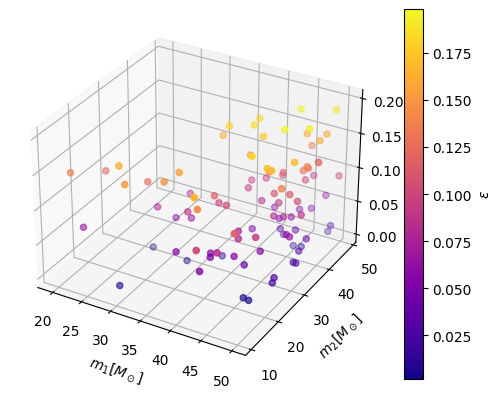
\includegraphics[width=0.45\textwidth]{paper/figures/pop3d0.2.png}
\caption{\label{fig:pop3d0.2} Synthetic Population of EBBHs. The left figure represents the population for $\sigma_\epsilon=0.05$ and right figure represetns the population for $\sigma_\epsilon=0.1$}

\end{figure}


\subsection{Scaled Population}

To compare the synthetic EBBHs population with the non-eccentric BBHs (NEBBHS), we created four more populations by scaling the existing populations using the Eq. \ref{eq:scaling} defined in \cite{2021_scaling_paper}. The Eq. \ref{eq:scaling} removes the eccentric component from the population, scales the masses, and eventually, we get non-eccentric populations to compare with the existing eccentric population.
\begin{align}
\label{eq:scaling}
M^{ecc} = \frac{M}{(1-\frac{157}{24}\epsilon^2)^{3/5}}
\end{align}




\begin{table*}[]
    \centering
    \begin{tabular}{|ccccccc|}
        \hline
        $\sigma_\epsilon$ & $m^1_{min} [M_\odot] $ & $m^1_{max} [M_\odot]$ & $m^2_{min} [M_\odot]$ & $m^2_{max} [M_\odot]$ & $\epsilon_{min}$ & $\epsilon_{max}$\\ \hline
        0.05 & 16.68 & 49.64 & 10.77 & 46.75 & 0.01 & 0.05\\ \hline
        0.1 & 18.95 & 49.51 & 9.89 & 48.33 & 0.05 & 0.1\\ \hline
        0.15 & 9.13 & 49.55 & 9.1 & 49.11 & 0.1 & 0.15\\ \hline
        0.2 & 18.2 & 49.79 & 10.3 & 47.08 & 0.15 & 0.2\\ \hline
    \end{tabular}
    \caption{Scaled Population Properties}
    \label{tab:popscl_prop}
\end{table*}
 

\begin{figure*}

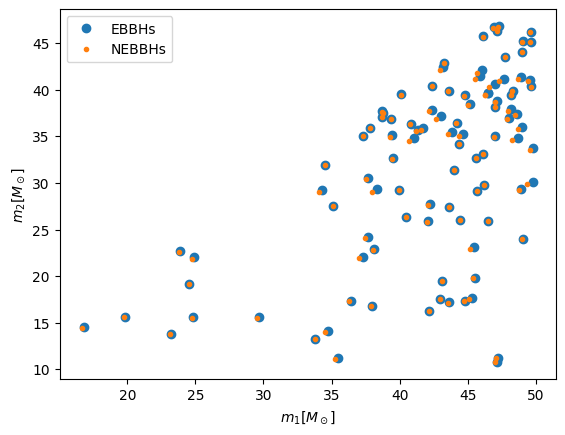
\includegraphics[width=0.45\textwidth]{paper/figures/pop0.05.png}
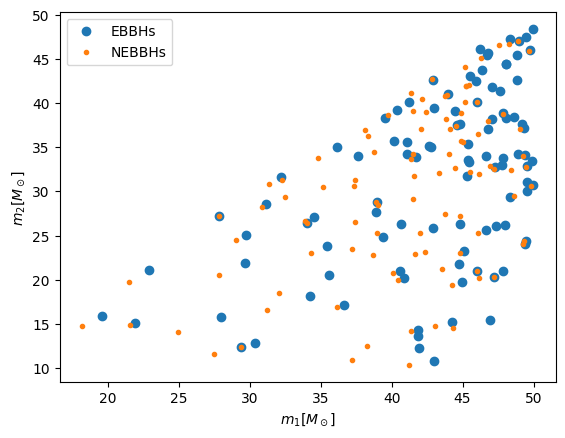
\includegraphics[width=0.45\textwidth]{paper/figures/pop0.2.png}
\caption{\label{fig:pop_0.05_0.2} The left figure shows the primary mass vs secondary mass of the EBBHs and NEBBHs with $\sigma_\epsilon =0.05$. The right figure shows the same plot but for $\sigma_\epsilon=0.2$} 

\end{figure*}




To get the non-eccentric population, we apply the Eq. \ref{eq:scaling} on the population given in Fig. \ref{fig:pop2d05} and get the new population with scaled masses. We get the new minimum and maximum values for the primary and secondary masses in Fig. \ref{fig:pop2dscal05}. 
   


The significant effect after the scaling is not only the mass shift, but one may notice in Fig. \ref{fig:pop2dscal05} that $14$ sources were missed out of $100$. This reflects that we may miss the various sources by ignoring the effect of eccentricity. The mass scaling effect is visible in Fig. \ref{fig:pop2d05diff}, and we also notice that sources start missing after $e \gtrsim 0.38$.













 
   

                            

\section{Results}

we can discuss the corner plots here.

\begin{figure*}

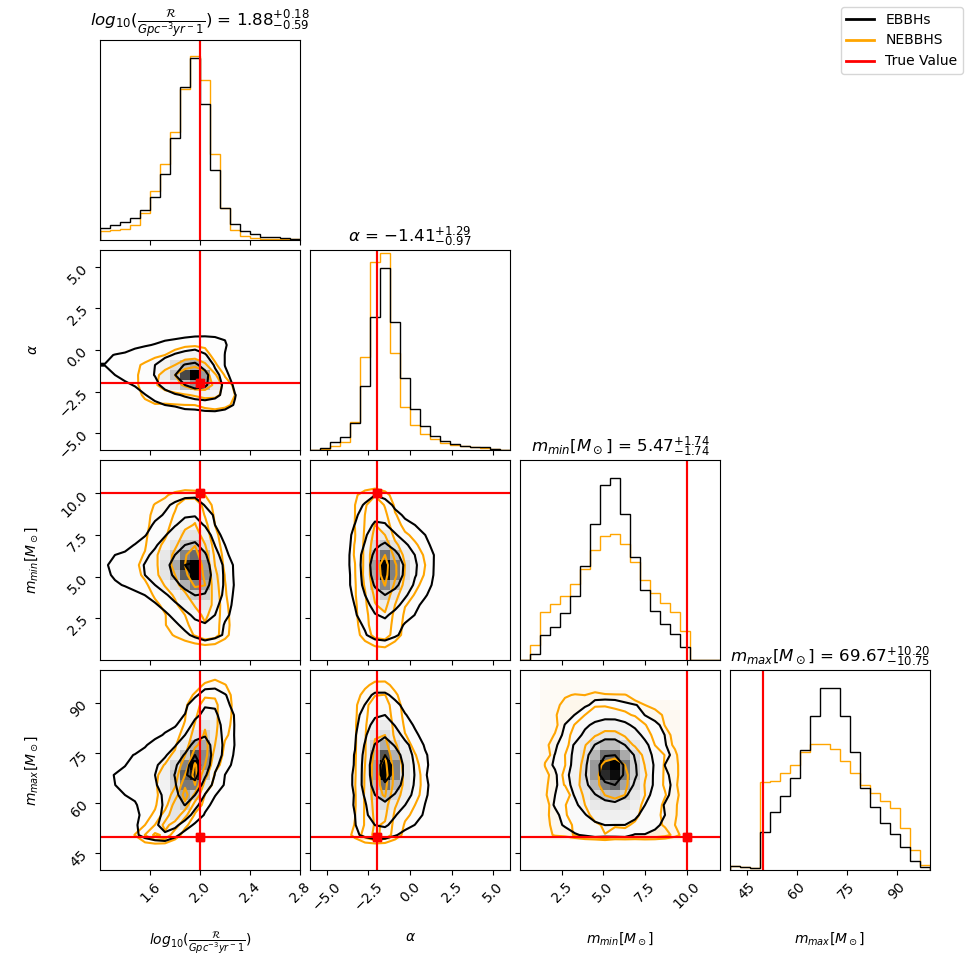
\includegraphics[width=0.95\textwidth]{paper/figures/corfig_0.05.png}
\caption{\label{fig:pop3d05}\textbf{Corner Plots for EBBHs and BBHS with $\sigma_\epsilon=0.05$}}

\end{figure*}
Same population.
\begin{figure*}

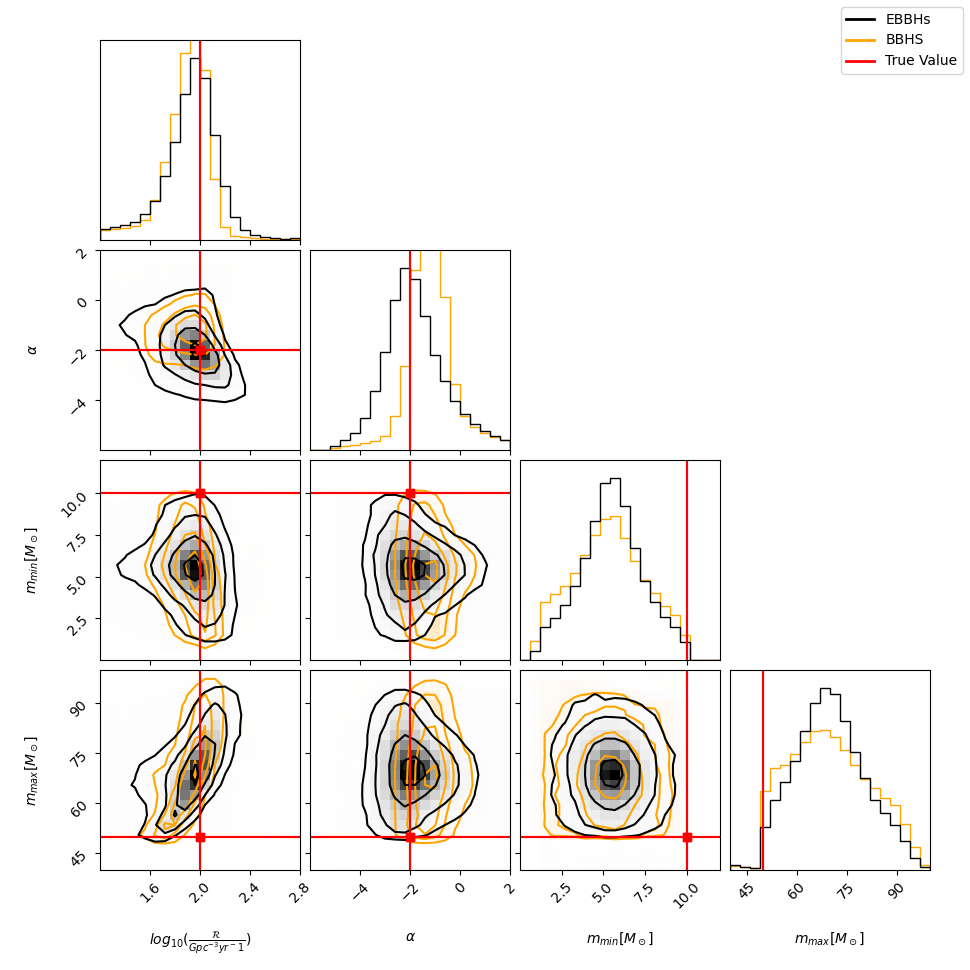
\includegraphics[width=0.95\textwidth]{paper/figures/corfig_0.2.png}
\caption{\label{fig:pop3d05}\textbf{Corner Plots for EBBHs and BBHs with $\sigma_\epsilon=0.2$}}

\end{figure*}

Need to write it later. 







% \begin{align} \label{eq:strain_mode}
% h(t,\vartheta,\phi;\bm{\lambda}) = 
% \sum_{\ell=2}^{\infty} \sum_{m=-\ell}^{\ell} \frac{D_{\rm ref}}{D} h^{\ell m}(t;\bm{\lambda}) \Y{-2}_{\ell m} \left(\vartheta, \phi \right) \, ,
% \end{align}


% \begin{widetext}
% \begin{align}
% \ln {\cal L}(\bm{\lambda}, \theta) 
% &= (D_{\rm ref}/D) \text{Re} \sum_k \sum_{\ell m}(F_k \Y{-2}_{\ell m})^* Q_{k,lm}(\bm{\lambda},t_k)\nonumber \\
% &   -\frac{(D_{\rm ref}/D)^2}{4}\sum_k \sum_{\ell m \ell' m'}
% \left[
% {
% |F_k|^2 [\Y{-2}_{\ell m}]^*\Y{-2}_{\ell'm'} U_{k,\ell m,\ell' m'}(\bm{\lambda})
% }
% % \right. \nonumber \\ & \left.
%  {
% +  \text{Re} \left( F_k^2 \Y{-2}_{\ell m} \Y{-2}_{\ell'm'} V_{k,\ell m,\ell'm'} \right)
% }
% \right]
% \label{eq:def:lnL:Decomposed}
% \end{align}
% \end{widetext}

% \begin{eqnarray}
% {\cal L}_{\rm margT} \equiv  \int {\cal L} \frac{dt}{T}
% \label{eq:lnL:tmarg}
% \end{eqnarray}












% \begin{table*}
% \begin{tabular}{lrr|ccccc|rr}
% Version & srate & modes & $\tau_{start}$ & $\tau_{setup}$ & $\tau_{ad}$ & $\tau_{it,like}$ &$\tau_{it,rest}$ &
% $\frac{T_{ILE}}{N_{eval}}$ & GPU \\  %\hline 
%   &   Hz & m & sec & sec & & $\mu$sec & $\mu$sec  &sec  & use  \%\\ \hline 
% % ~/parse_report.sh profile_nogpu_pcdev13.log | more
% CPU & 16384 & $\pm 2 $ & 20 & 2.4 &&540 & 20 &  690  \\ 
%        & 4096 & $\pm 2 $ &   20  &&&& 20 \\ \hline
% % ./parse_report.sh 20190130-profile_nogpu_HM_pcdev13.log  | more
% % /parse_report.sh ./profile_nogpu_HM_lowres_pcdev13.log 
% %    setup time: PrecomputeLikelihoodTerms, includes waveform generation. 
% %   evaluation: FactoredLogLikelihodTimeMarginalized Divide by actual number of calls, since not a block!
% %    
% CPU & 16384 & $\pm 2,\pm 1 $ & 20 & 1.5 && 680 & 20 &  1060  \\ 
%        & 4096 & $ \pm 2, \pm 1 $ &   20 &&&& 20  \\ \hline

%GPU (a) & 16384 & $\pm 2 $  & 20  & & && & 270 \\
%            & 4096 &$\pm 2 $  &  20 &  & & & & 45 \\ \hline

%GPU (b) & 16384 & $\pm 2$ & 20  & 1.8 & 1 & 0.85& 20 &28 & 15\\
%        & 4096 & $\pm 2$  & 20 & $1.2 $ &  1  & 0.75 & 20  & 25\\ \hline

% GPU (b) & 16384 & $\pm 2, \pm 1$ & 20 & 1 && 4.2 & 20  & 38  \\
%        & 4096 & $\pm 2, \pm 1$ & 20 & 1&& 2.5  & 20 & 35 & \\ \hline

% GPU (c) & 16384 & $\pm 2 $  & 20  &6  & & 18&  58&160 &  \\
%             & 4096 &$\pm 2 $  &  20 & 3.7 & & 11  & 58  & 140 & $\simeq 50$ \\
% \end{tabular}
% Compute node at LIGO-WA
% \caption{\label{tab:CostBreakdown}\textbf{Profiling performance: Binary black holes}: Evaluation costs for the
%   marginalized likelihood on default
%   hardware, for a two-mode system $(l,m)=\pm 2$ analyzing $T=8\unit{s}$ of data with a massive binary black hole
%   $m_1=35 M_\odot,M_2=30 M_\odot$.  The last column indicates peak GPU utilization.
% }
%\end{table*}










% \subsection{Binary black hole analysis}
% \label{sec:sub:BBHFull}

% \begin{figure*}

% 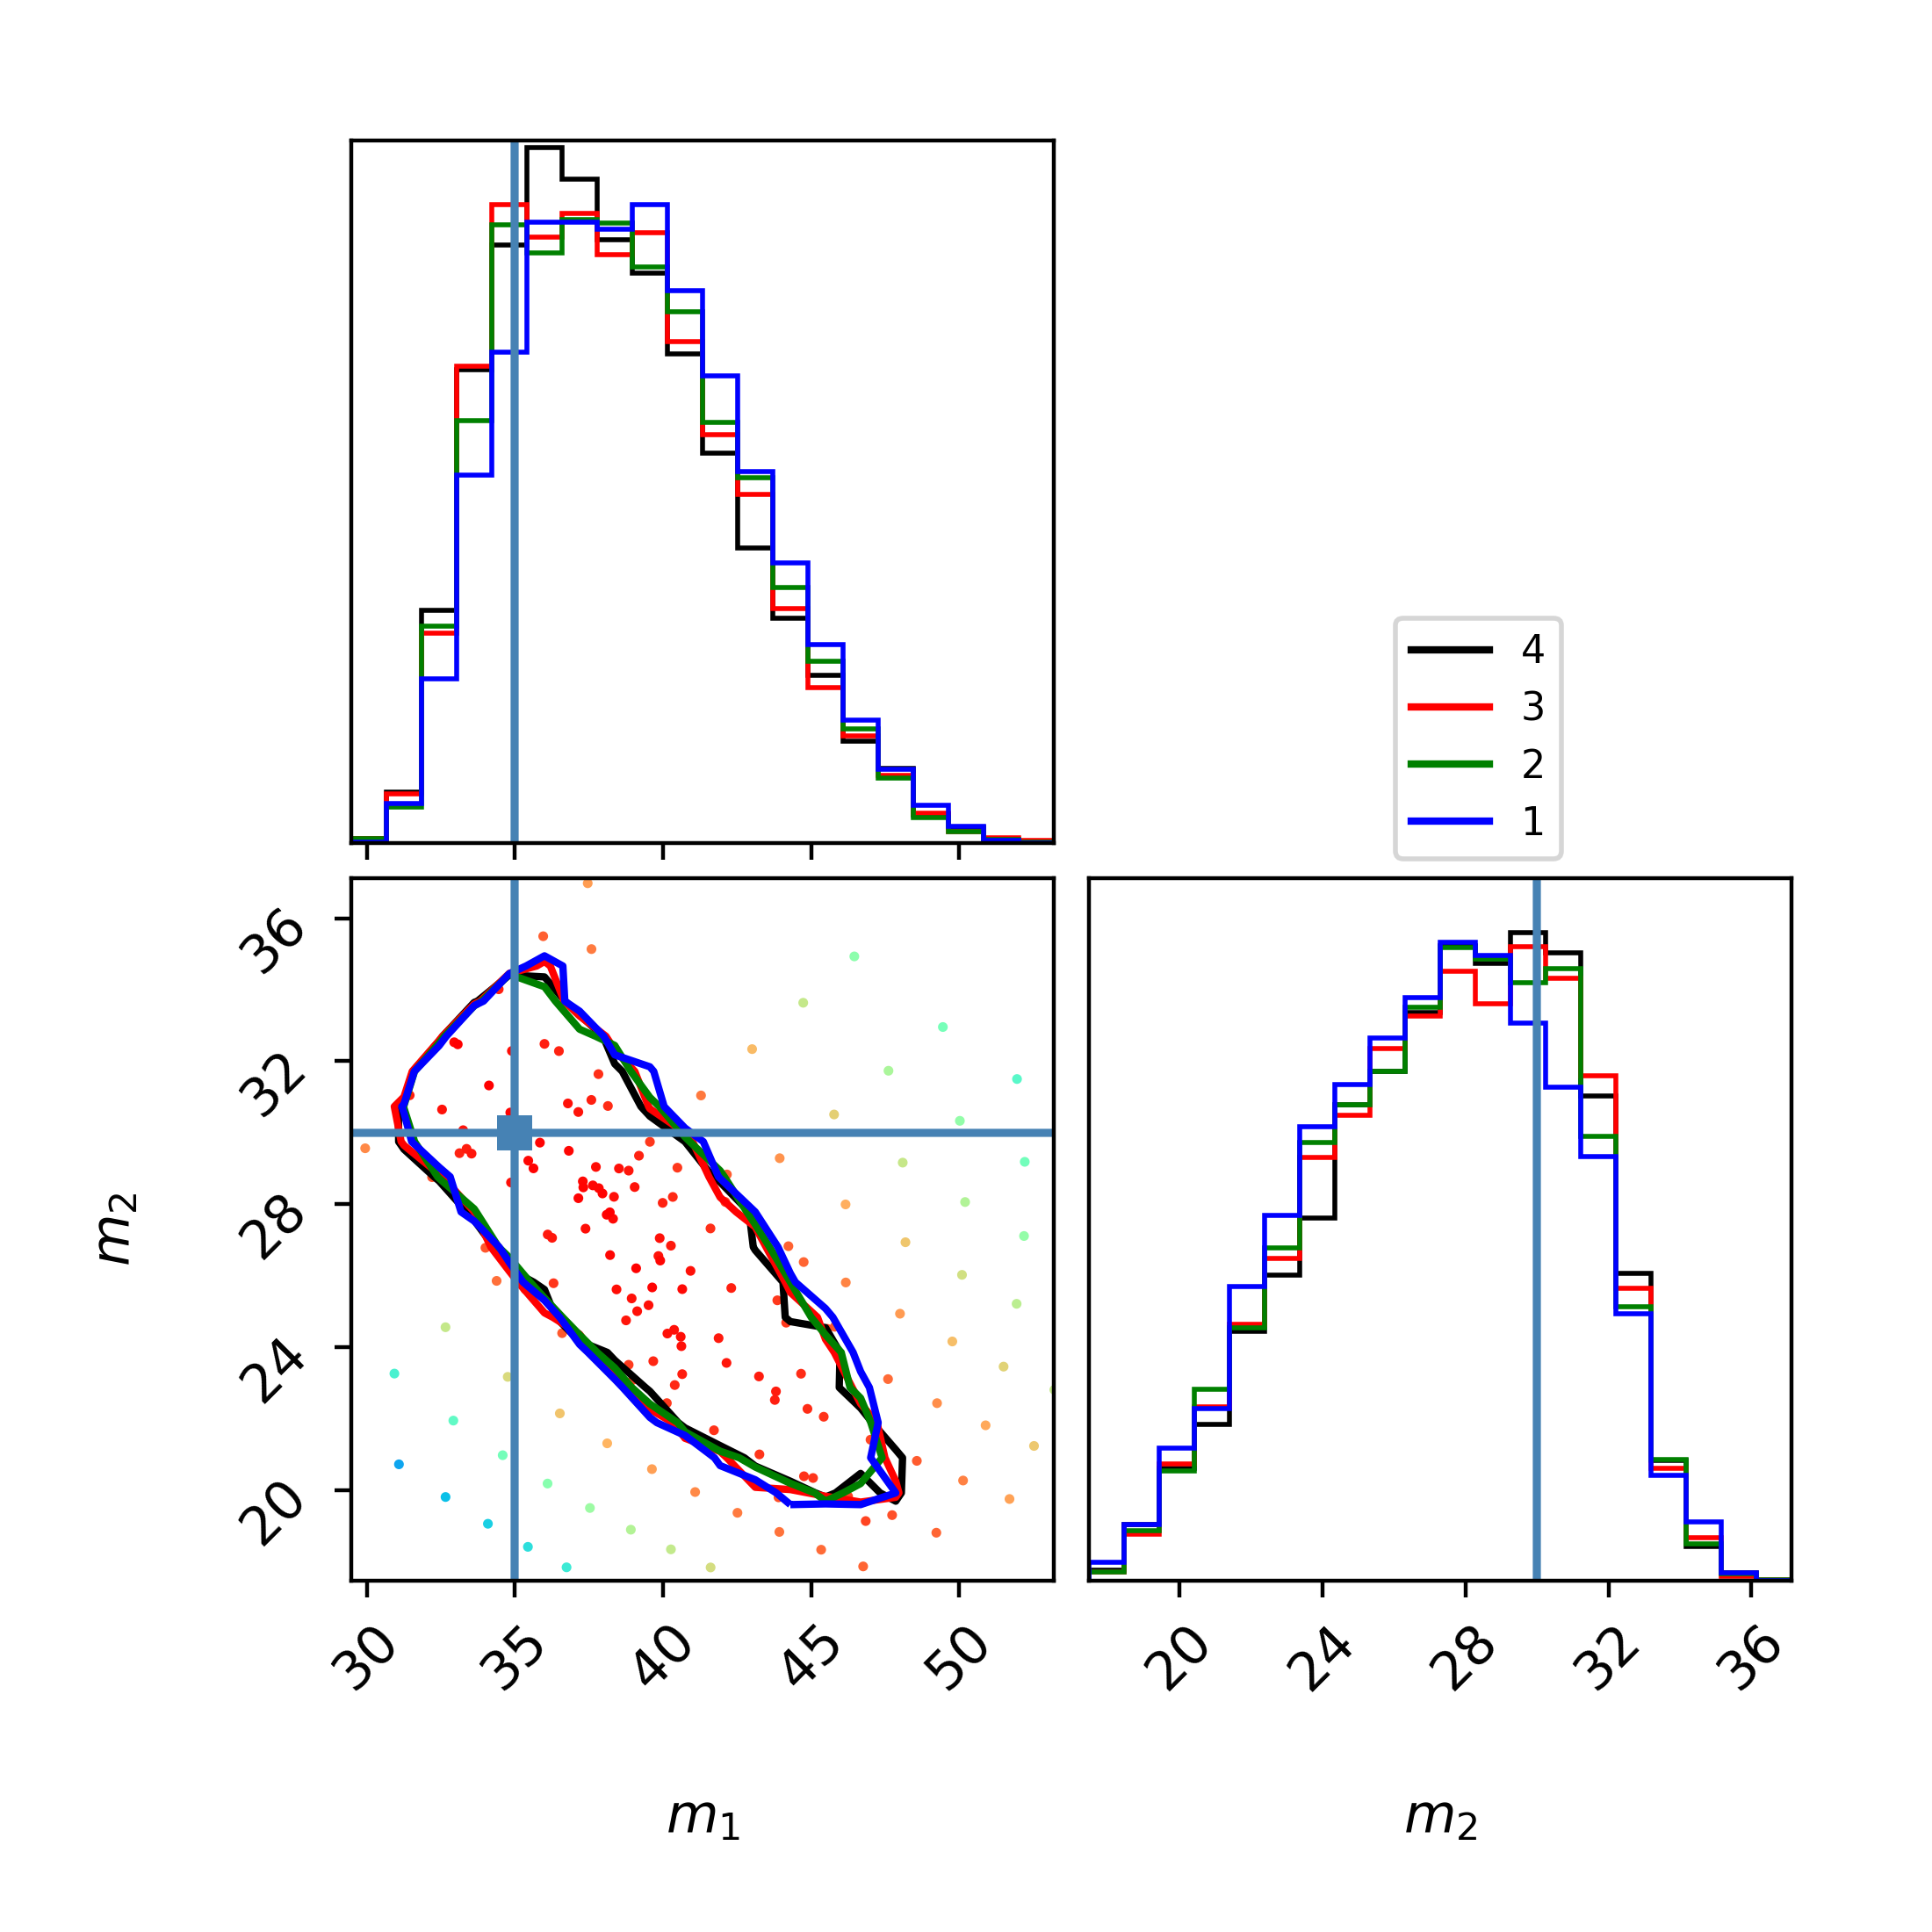
\includegraphics[width=0.45\textwidth]{figures/bbh_zerospin_m1_m2.png}
% 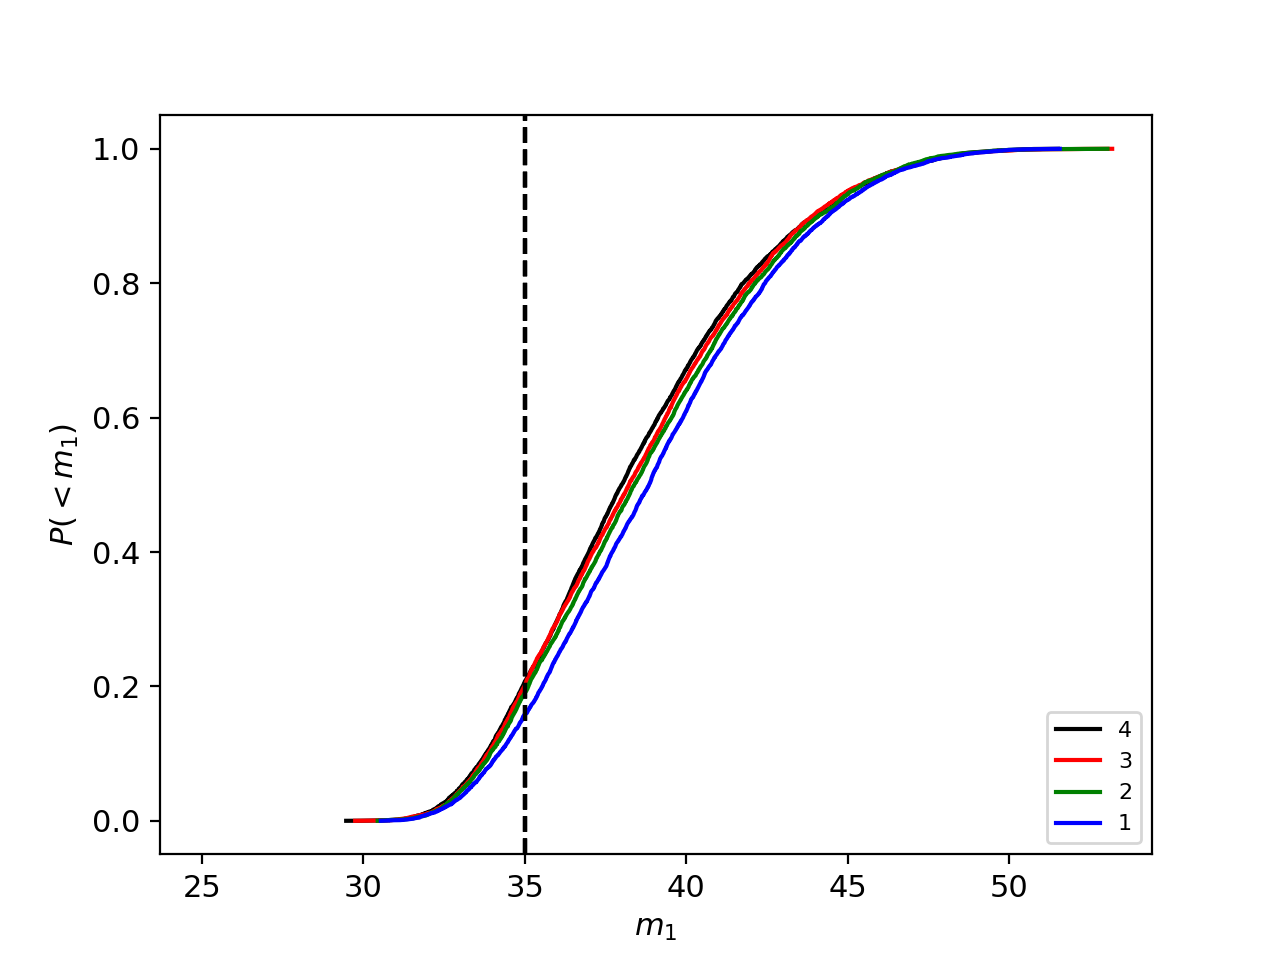
\includegraphics[width=0.45\textwidth]{figures/bbh_zerospin_m1_cum.png}
% % python plot_mean_variance.py --convergence-file 20190203-bbh-zerospin-batch_gpu_lowlatency_meanVar.dat  --output bbh_zerospin_lnL_meanVar
% 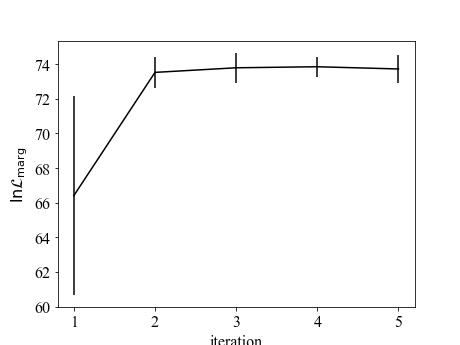
\includegraphics[width=0.45\textwidth]{figures/bbh_zerospin_lnL_meanVar.png}
% % python plot_convergence.py --convergence-file 20190203-bbh-zerospin-batch_gpu_lowlatency.dat
% 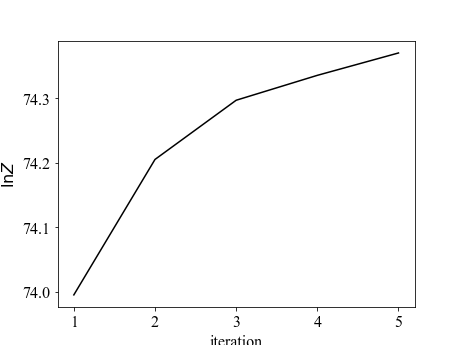
\includegraphics[width=0.45\textwidth]{figures/bbh_zerospin_lnL_converge.png}
% \caption{\label{fig:BBH:MultiIterate}\textbf{Convergence of BBH analysis: Zero spin}: Results for marginal posterior distributions
%   of our fiducial synthetic binary black hole.  Solid contours show credible intervals; solid one-dimensional distributions
%   show marginal CDFs and PDFs for the corresponding variable; and colored points indicate the location $\bm{\lambda}$ and
%   value of the underlying marginalized likelihood evaluations.   
% %The corresponding dotted curves show an analysis using   only the $m=\pm 2$ modes \editremark{perform both} 
% \emph{Left panel } Posterior distribution
%   over  $\mc$ and
%   $\delta=(m_1-m_2)/M$.    \emph{Right panel}: Marginal 1d CDFs of $\mc$, showing convergence.
% \emph{Bottom left}: Mean and variance of  \AddedResponse{the array $\ln{\cal L}_{\rm marg}(\bm{\lambda}_j)$  for
% $j=1,2,\ldots N_{\rm eval}$ indexing all candidate sets of intrinsic parameters $\bm{\lambda}_j$ performed in that iteration},  showing that after the
% first iteration the
% candidate points are consistent with the posterior (i.e., no proposed point has very low $\ln {\cal L}_{\rm marg}$).
% \emph{Bottom right panel}: The estimated evidence $Z = \int d\bm{\lambda} {\cal L}_{\rm marg}$ versus iteration number.  As systematic fitting error dominates our
% error budget, Monte Carlo error is not shown.
% }
% \end{figure*}


















\section{Conclusions}
\label{sec:conclude}
In Progress, 













\begin{acknowledgements}
We thank our anonymous referee for the helpful feedback.

\end{acknowledgements}


\appendix
In Progress,




%\bibstyle{unsrt}
\bibliography{paperexport,LIGO-publications}
\end{document}
